% Phase 1: empirical diagnostics on S&P 500 returns

\section{Empirical diagnostics on S\&P~500 daily returns}\label{sec:diagnostics}

\paragraph{Dataset.} We pull adjusted close prices for the S\&P~500 constituents from
$2016$-$05$-$11$ to $2026$-$05$-$07$ via \texttt{yfinance}, drop tickers with more than
$5\%$ missing observations or fewer than two years of history, and keep $n=468$ stocks
over $T=2{,}512$ trading days. The resulting log-return matrix $R\in\mathbb R^{T\times n}$ has aspect
ratio $n/T=0.186$. We compute the sample mean $\hat\mu := \tfrac1T\sum_t R_{t,:}$ and
sample covariance $\hat\Sigma := \tfrac1T R^\top R - \hat\mu\hat\mu^\top$ on the first
$80\%$ of the window (a $T_{\mathrm{tr}}=2009$-day train block); the held-out $20\%$ is reserved
for out-of-sample Sharpe assessments later. The notebook \texttt{extract\_data.ipynb} produces
the cleaned panel and writes \texttt{data/returns.npy}.

\paragraph{Why diagnostics matter.} The portfolio-selection problem is one of \emph{discrete
optimization on noisy data}. Whether a particular algorithm or theoretical bound applies
depends on (i) the tail behaviour of $\hat\mu_i$, which controls Bonferroni and Bernstein
concentration; (ii) the spectrum of $\hat\Sigma$, which controls the Marchenko-Pastur (MP)
edge and the strength of the dominant factor; and (iii) the Restricted Isometry Property
(RIP) of $\hat\Sigma$, which controls when convex relaxations are equivalent to the
combinatorial problem. We characterise all three on the train block.

\subsection{Sub-Gaussian / sub-exponential norms}\label{ssec:psi}

For each stock $i$ we estimate the Orlicz norms
$\|R_{:,i}\|_{\psi_2} := \inf\{c>0: \mathbb E[\exp(R_{:,i}^2/c^2)]\le 2\}$ and
$\|R_{:,i}\|_{\psi_1} := \inf\{c>0: \mathbb E[\exp(|R_{:,i}|/c)]\le 2\}$ via the standard
empirical-moment estimator on standardised returns \cite{lec:subexp}. Both norms are \emph{finite for every
stock} (i.e., the empirical moment-generating function exists at the canonical scale on
all $i$): we obtain median $\|\cdot\|_{\psi_2}=3.63$ vs.\ Gaussian reference $1.63$, and
median $\|\cdot\|_{\psi_1}=1.66$ vs.\ Laplace reference $1.44$.

\noindent\emph{Implication.} The data are sub-Gaussian but with $\psi_2$ inflated by a
factor of roughly $2\times$ over the Gaussian benchmark. This puts us squarely in the
Bernstein regime \cite{lec:concentration}: any concentration argument we deploy (e.g., for max-norm of $\hat\mu$ or
for entrywise covariance bounds) carries an effective variance proxy
$\hat\nu^2 \approx (3.63/1.63)^2 \cdot \nu_{\mathrm{Gaussian}}^2 \approx 5\,\nu_{\mathrm{Gaussian}}^2$.
We will use $\hat\nu$ to instantiate the recovery threshold of
Theorem~\ref{prop:slh-recovery} on real data.

\begin{figure}[ht]
\centering
\begin{minipage}{0.48\textwidth}\centering
  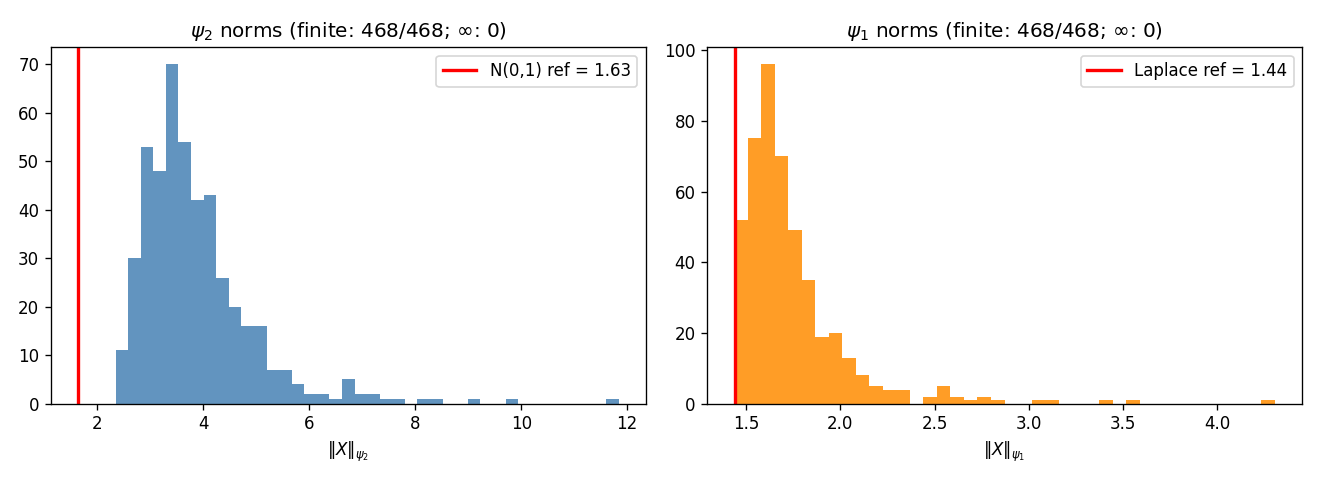
\includegraphics[width=\linewidth]{figs/psi_norms.png}
  \subcaption{Distribution of empirical $\|\cdot\|_{\psi_2}$ and $\|\cdot\|_{\psi_1}$ across the $n=468$ stocks; Gaussian and Laplace references shown as vertical lines.}\label{fig:psi-norms}
\end{minipage}\hfill
\begin{minipage}{0.48\textwidth}\centering
  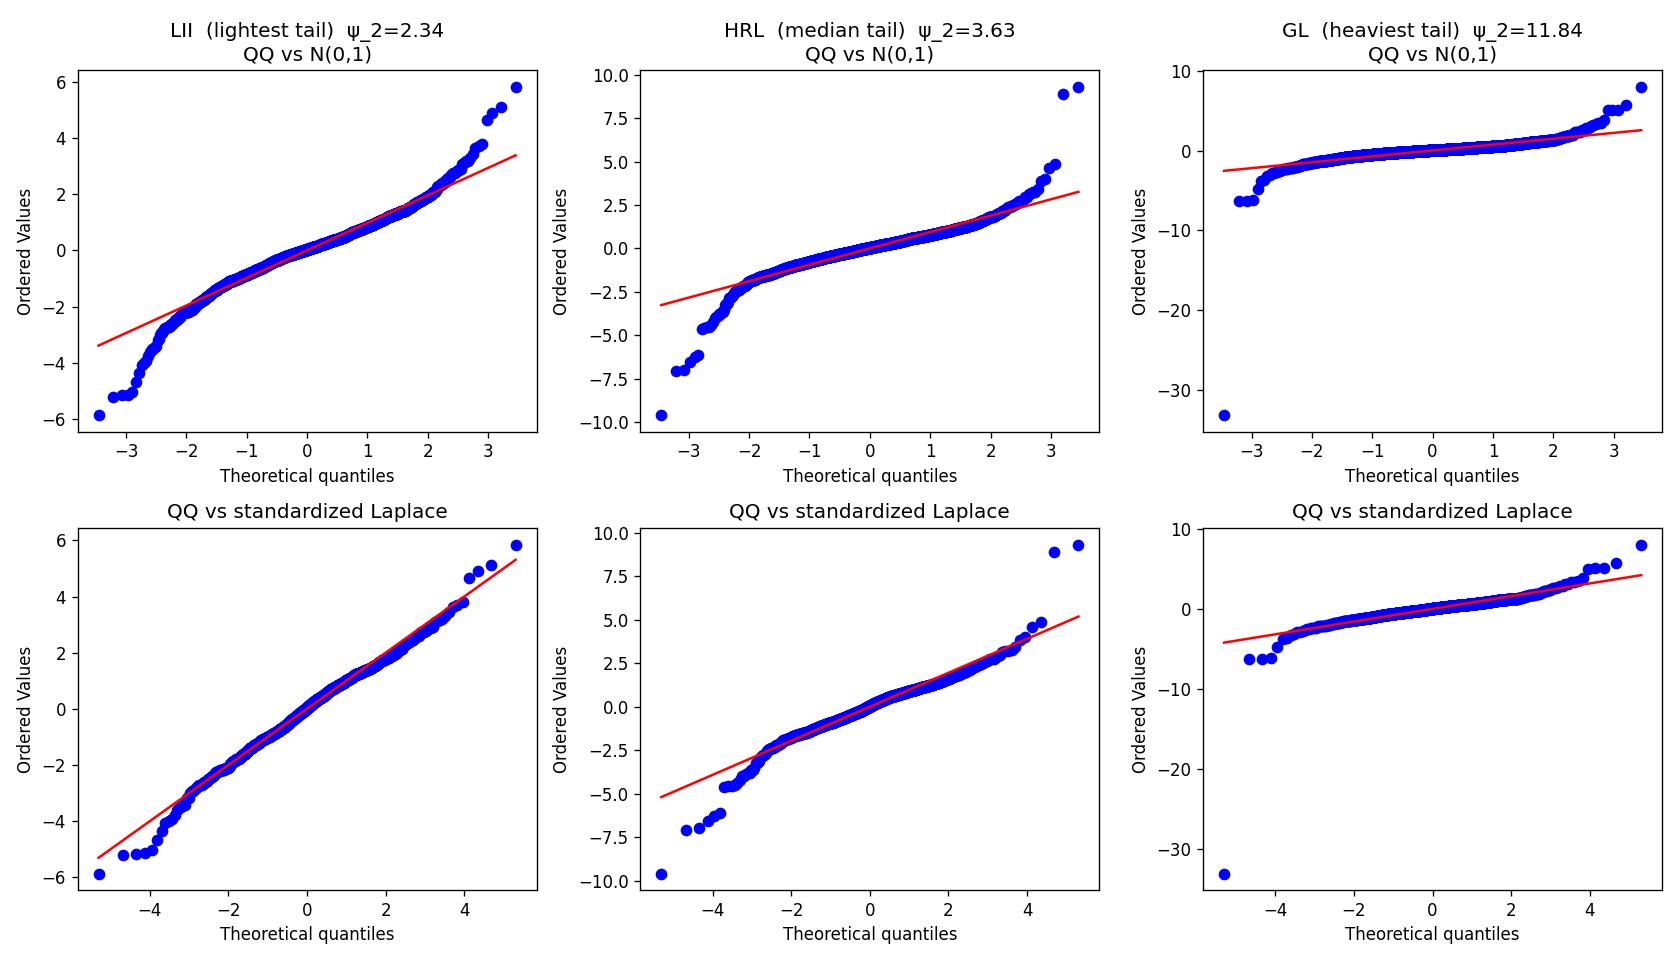
\includegraphics[width=\linewidth]{figs/qq_plots.png}
  \subcaption{Q-Q plots of standardised returns vs.\ Gaussian and Laplace quantiles for six representative stocks.}\label{fig:qq}
\end{minipage}
\caption{Tail diagnostics. The data are sub-Gaussian (every stock has finite $\psi_2$) but visibly fatter-tailed than Gaussian, sitting between the Gaussian and Laplace reference distributions.}\label{fig:tails}
\end{figure}

\subsection{Spectral structure of $\hat\Sigma$}\label{ssec:spectrum}

For the empirical covariance with $n/T=0.186$ the Marchenko-Pastur edges \cite{lec:rmt} (under iid
isotropic returns of unit variance, rescaled to the empirical trace) are
$\lambda_\pm = (1\pm\sqrt{n/T})^2 = (1\pm 0.4316)^2$ scaled by
$\bar\sigma^2 := \tfrac1n\,\mathrm{tr}(\hat\Sigma)$. Concretely
$\lambda_+ = 7.28\!\times\!10^{-4}$ (in daily-return units squared).
The top sample eigenvalue is $\lambda_{\max}(\hat\Sigma) = 7.01\!\times\!10^{-2}$, i.e.,
\[
  \frac{\lambda_{\max}(\hat\Sigma)}{\lambda_+}
   \;=\; 96.3,
\]
$32$ eigenvalues exceed the MP edge, and the top $10$ eigenvalues account for $53.1\%$ of
$\mathrm{tr}(\hat\Sigma)$. The largest eigenvector is dominated by uniformly-positive
loadings: the empirical \emph{market factor}. We henceforth treat $\hat\Sigma$ as a
factor-plus-noise object,
\begin{equation}\label{eq:factor-noise}
  \hat\Sigma \;\approx\; \sum_{j=1}^{r} \lambda_j\, v_j v_j^\top \;+\; \nu^2 I_n,
  \qquad r\in[5,32],
\end{equation}
i.e., a Wishart bulk plus a low-rank deterministic spike in the random-matrix
sense. This justifies the ridge regularisation in stage~(S1) of \textsc{Slh}\
(\S\ref{sec:slh}): the spectral-aware step
$(\gamma\hat\Sigma + \eta I)^{-1}\hat\mu$ inverts the factor part cleanly while the
$\eta\, I$ term tames the bulk.

\begin{figure}[ht]
\centering
\begin{minipage}{0.48\textwidth}\centering
  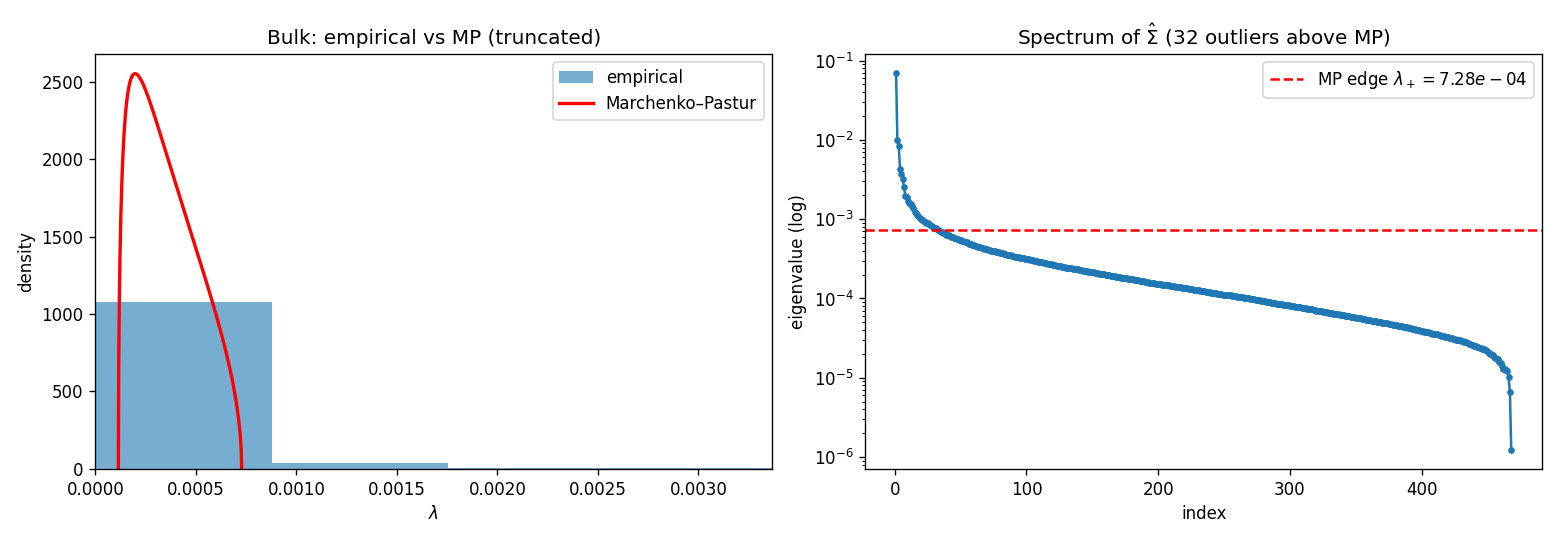
\includegraphics[width=\linewidth]{figs/spectrum_vs_mp.png}
  \subcaption{Empirical eigenvalue distribution of $\hat\Sigma$ (histogram) overlaid with the Marchenko-Pastur density (red) at aspect ratio $n/T=0.186$. The bulk matches MP; $32$ outliers (top tail) are visible to the right of $\lambda_+$.}\label{fig:spectrum}
\end{minipage}\hfill
\begin{minipage}{0.48\textwidth}\centering
  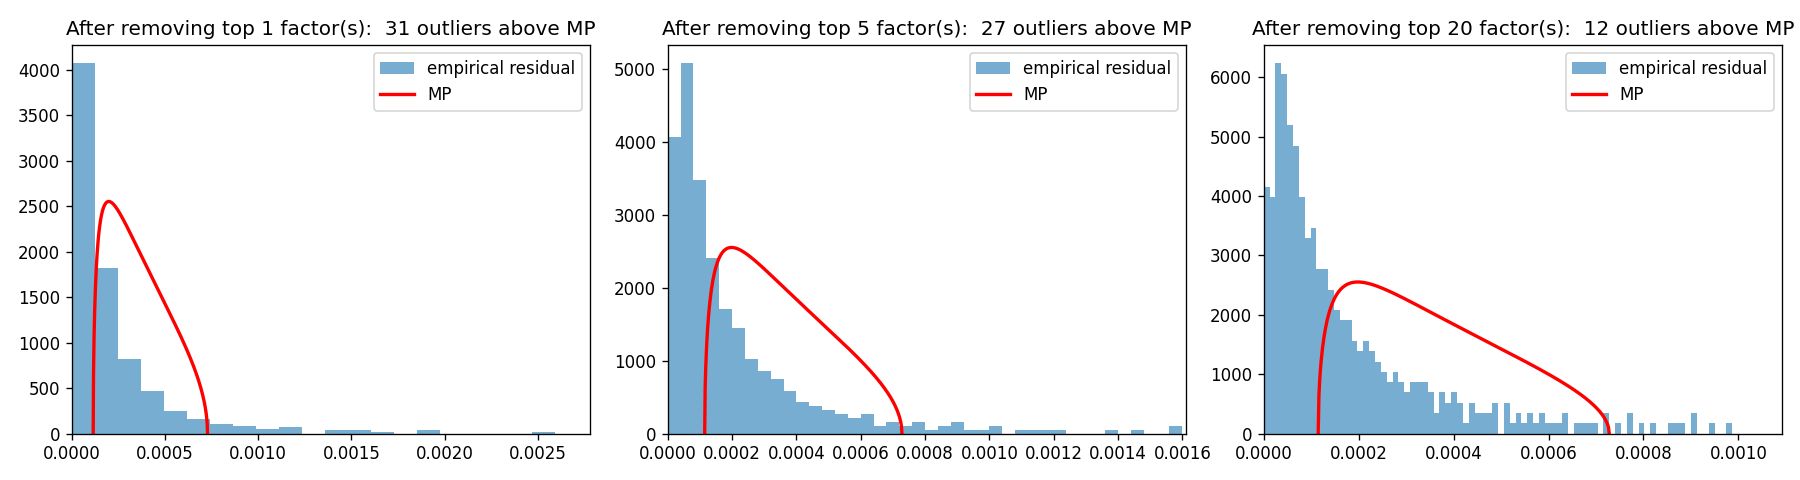
\includegraphics[width=\linewidth]{figs/residual_spectrum.png}
  \subcaption{Eigenvalue spectrum of the factor-residualised covariance $\hat\Sigma_\perp$ after removing the top $r{=}5$ factors. The residual has bulk much closer to the MP prediction.}\label{fig:residual-spectrum}
\end{minipage}
\caption{Spectral structure of $\hat\Sigma$. The empirical covariance is dominated by a market factor and $\sim\!30$ outlier eigenvalues; the residual after factor projection looks much more like a random Wishart matrix.}\label{fig:spectrum-pair}
\end{figure}

\subsection{Failure of the Restricted Isometry Property}\label{ssec:rip}

For the LASSO-Markowitz baseline (\S\ref{sec:lasso}) to provably recover the true sparse
support one wants $\hat\Sigma$ to satisfy a Restricted Isometry Property (RIP) \cite{lec:cs}. The
standard $k$-RIP constant is
\[
  \delta_k(\hat\Sigma) \;:=\; \sup_{|S|\le k}\,\big|\lambda_{\max}(\hat\Sigma_{S,S}) - 1\big| \;\vee\;
                              \big|\lambda_{\min}(\hat\Sigma_{S,S}) - 1\big|,
\]
after re-scaling so that $\mathrm{diag}(\hat\Sigma) = 1$. Sample-splitting and Monte-Carlo
estimation over $10^4$ random $k$-subsets gives the following $95$-th-percentile values
of $\delta_k$:
\[
  \delta_5 \approx 0.846,\qquad \delta_{10} \approx 0.867,\qquad \delta_{20} \approx 1.045,
  \qquad \delta_{50}\approx 0.853.
\]
LASSO's exact-recovery analysis requires $\delta_{2k}<\sqrt 2 - 1\approx 0.414$;
here $\delta_k$ already exceeds $1/3$ at the $95$-th percentile for every $k$.
\emph{RIP fails uniformly}, and we therefore expect LASSO-Markowitz to be a poor
recovery algorithm on this dataset, a prediction that Phase~2a confirms quantitatively.

\begin{figure}[ht]
\centering
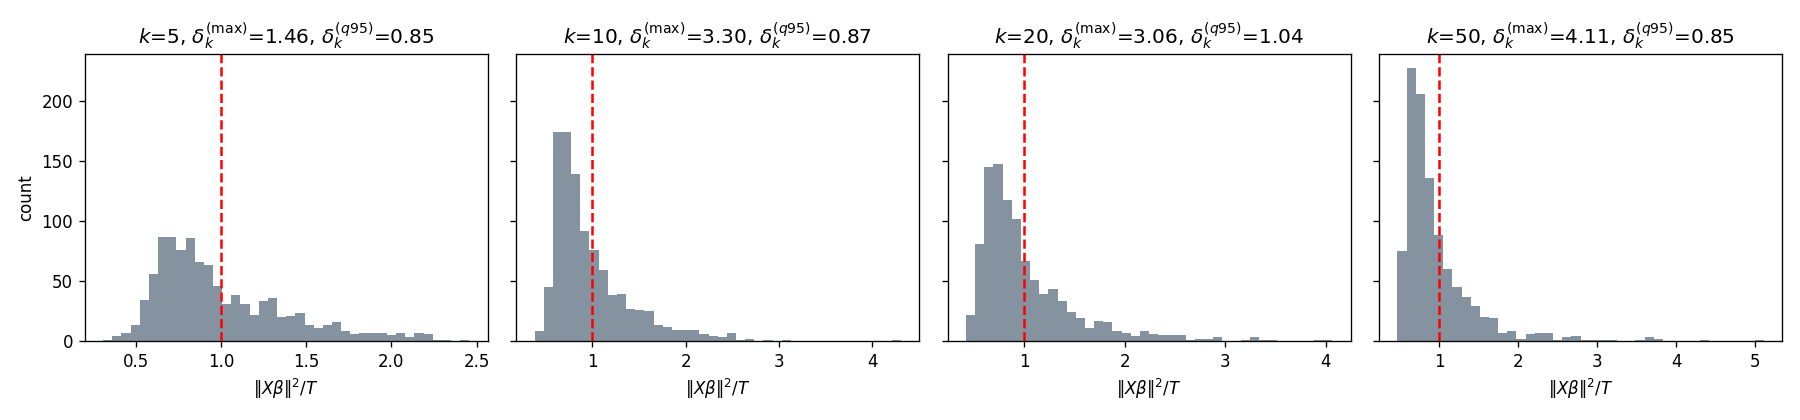
\includegraphics[width=0.7\textwidth]{figs/rip_probe.png}
\caption{Empirical RIP probe. For each $k\in\{5,10,20,50\}$ we evaluate $\delta_k$ on $10^4$ random subsets and show the median, $95$-th percentile, and maximum. The dashed line is the LASSO recovery threshold $\sqrt 2 - 1$. The $95$-th percentile exceeds the threshold for every $k$, so LASSO-Markowitz cannot be expected to recover the combinatorial optimum.}\label{fig:rip}
\end{figure}

\paragraph{Summary of Phase 1.} The S\&P data is sub-Gaussian (Bernstein-applicable);
$\hat\Sigma$ is dominated by a market factor plus $\sim\!30$ outlier eigenvalues; and RIP
fails. These three facts \emph{together} motivate the algorithmic design of \textsc{Slh}\
(spectral seed \emph{plus} combinatorial polish, rather than convex relaxation) and the
theoretical scope of Phase~3 (planted-spike model whose noise level $\nu$ is calibrated to
the residual variance $\hat\nu^2 \approx \tfrac{1}{n}\mathrm{tr}(\hat\Sigma_{\perp})$
after factor projection).
